\section {Implementation}

\subsection{Prototype}

We have  an in-kernel  data  plane  and user  space control/management
plane via TCP/UDP sockets, with a total of about 4000 lines of code in
C  and   C++.   There are    three  different options   for  in-kernel
implementation of the data plane: (i) OS  native  network stack; (ii) NIC
driver (e.g.,  DPDK~\cite{dpdk});   and  (iii)   customized  in-kernel
software switch (e.g.,  openvswitch~\cite{ovs}).  We choose option (i)
due to (a) \system has  to choose a  right interface before sending to
the driver   when  having  multiple  interfaces;  and  (b)  customized
in-kernel software switch has high overhead.  We use kernel modules to
register callback  functions with  Linux  \texttt{netfilter}  for data
plane operation. The   control/management  plane  has  an   extensible
complex control logic, and the data plane does specific simple actions
(e.g.,  header rewriting, queuing  to packets  user  space and  update
kernel hash table).  The user and the kernel  agent  communicate via 
\texttt{netlink}, a native   Linux  Inter Process Communication  (IPC)
function.  Currently the policy server  is   a simple TCP server  that
proactively pushes the policies to the agents.

\begin{figure}[ht]
\centering
% 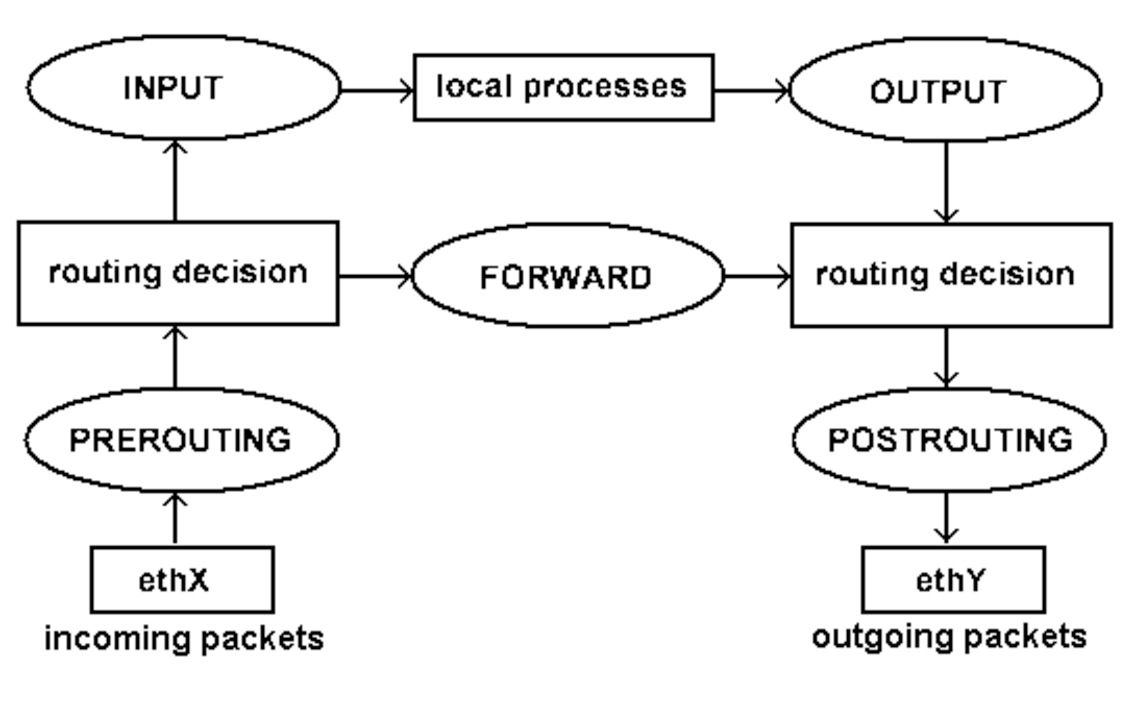
\includegraphics[scale=0.25]{figures/netfilter.pdf} 
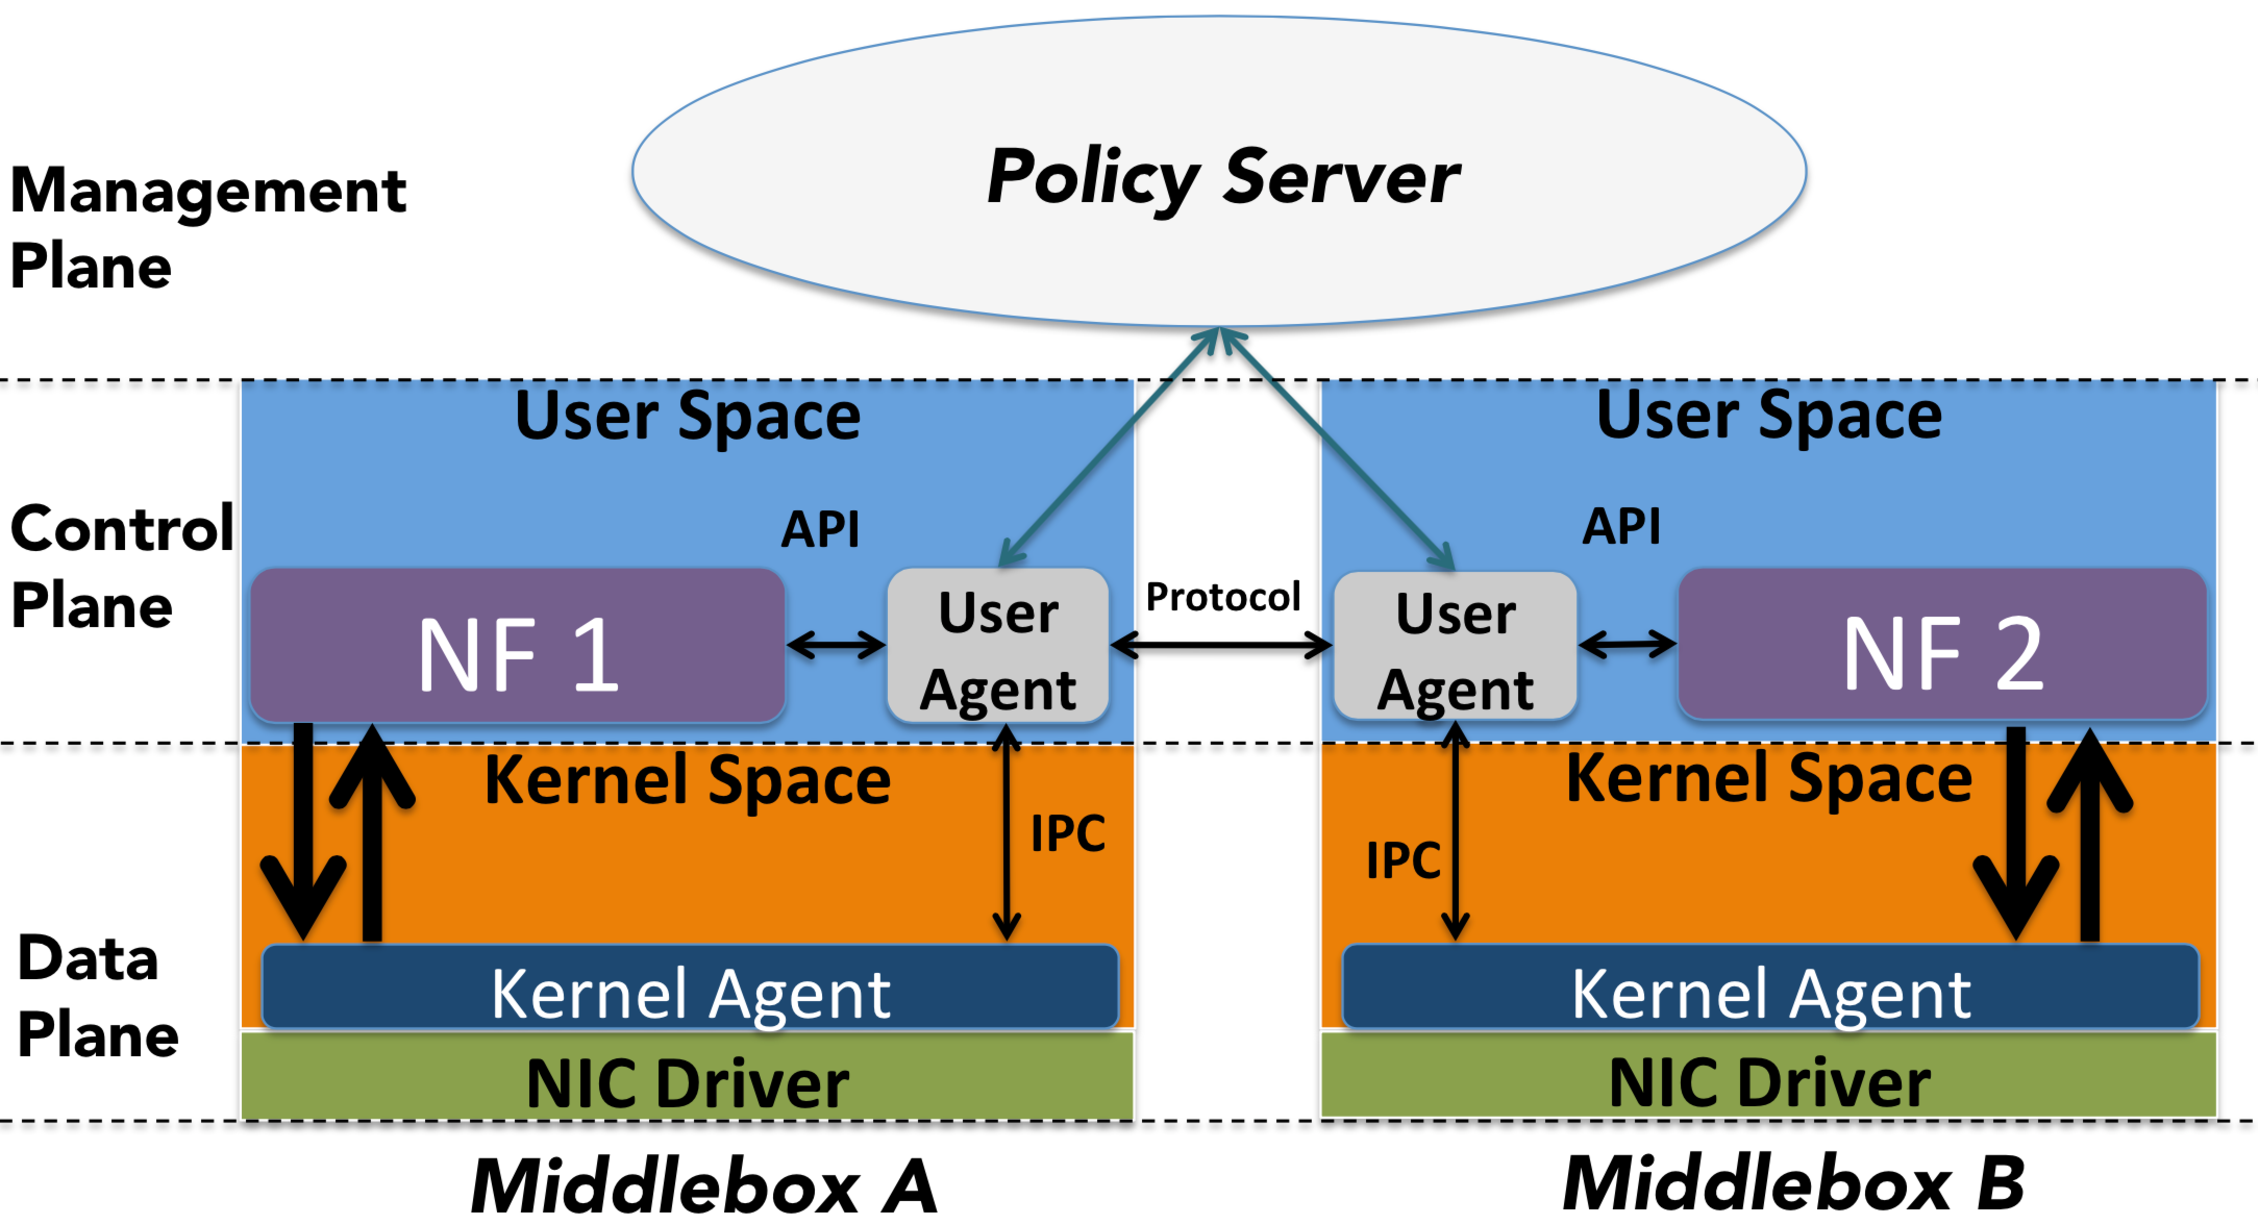
\includegraphics[width=\linewidth]{figures/archiIllustrrate.pdf} 

\caption{\small Layout of the implementation blocks}\label{netf}
\end{figure}





\subsection{Network Function Support}\label{sec:NFsupport}

We categorize NFs into two types --- active and passive functions --- based on whether the NF acts on the original packet. Table~\ref{nfhook} lists several commonly used NFs with the types, key functions to fetch session information and binding libraries. 

 Many passive NFs get a clone of the original packet and decide based on the copy. As described in \S\ref{sec:arch}, we restore the supersession header of the copy before delivering the packets to NF, so called vertical NAT. Based on Table~\ref{nfhook}, supersession restoring can be realized by extending libpcap~\cite{tcpdump} for a wide range of NFs. 



For active NFs, if they only act on the payload, supersession restoring also works. 
However, if the network function acts on the packet 5-tuple, we have to modify NF functions to notify the \system agent its own mapping. 
For example, a transparent cache proxy~\cite{squid} gets the packets from its listening port and sets up a new TCP socket to the final destination. \system will break the supersession into two if it is unware of the mapping between two sessions. On the other hand, if the NF informs the \system agent the mapping between its listening and sending TCP sockets, the \system agent can stitch the two together ``subsessions'' into one supersession. 
 


\begin{table}[t]\label{middleboxextension} 
\centering
 
\small
\begin{tabular} {|l |c |c |c|}
\hline

      Name          	  &         Type           & Key        	 &      Binding   \\
                      	  &                        &  Functions          &       Library  \\ \hline
PRADS~\cite{prads} (P) 	  &      Monitoring        &    got\_packet()      & libpcap   \\ \hline
Bro~\cite{bro} (P)      	  &      IDS               &   DumpPacket()      & libpcap   \\ \hline
Snort~\cite{snort} (P)  	  &        IDS         &    PQ\_Show()          & libpcap \\ \hline 
Balance~\cite{balance} (A)	  &      Load Balancer     &    recv(), writen()       &user socket\\ \hline
Squid~\cite{squid} (A) 	  &        Proxy           &  getsockopt()        & user socket  \\ \hline
Traffic   		  &    WAN-                &     net\_receive       &Linux  \\ 
Squeezer~\cite{tsqueezer} (A)&Optimizer &\_skb()   & skbuff \\ \hline


\end{tabular}
\caption{\small Popular Network Functions; (A) means active, (P) means passive NF. }\label{nfhook}
\end{table}


% \subsection{Middlebox Support}




% 
%Three way handshake
%read write lock
%kmalloc atomic for faster access
